\section{Comparison with \textit{Kiwi}'s \textit{Nomad}}
\label{sec:nomad}

At the present time, \textit{Kiwi}'s \textit{Nomad} is the only (non-disclosed) tool that is capable of addressing the formalized \textit{Flying Tourist Problem} in the form of an unconstrained multi-city routing problem, although limited to only 10 different nodes. To facilitate the comparison of the conceived optimization system with this tool, the definition of the user requests of the proposed FTP (see section \ref{sec:pf}) was kept as similar as possible to \textit{Kiwi}'s \textit{Nomad} interface. The user is asked to specify the departing/arriving city, together with the start date, the set of cities to be visited and the duration of the stay in each city.

The results provided by both applications were directly compared against each other, according to each considered objective function. The difference in the total flight price and duration (for each query) was also measured and analyzed as a function of the query parameters. The former evaluation will be called \textit{absolute comparison} (subsection \ref{sec:absolute_eval}), while the latter \textit{quantitative evaluation} (subsection \ref{sec:quantitative_eval}).

The execution of these tests involved over 100 different queries, by varying not only the number of nodes (2-10), but also the length of the trip start interval (1-15 days). All queries that were performed on both applications had its start and return city set to Lisbon (Portugal), while each city to be visited belongs to the same set of hub airports that were considered in the previous subsections.  These queries were executed during the period between 15 and 16 of June 2018 and the base start date was set to the 1st of August 2018, which, at the time of the tests, was 45 days in the future. The staying period in each city was set to a random value between 1 and 5 days. For extended start periods, the base start date was extended by 31 days.


\subsection{Absolute comparison}
\label{sec:absolute_eval}

Both applications respond to each query with three different sets of flights, serving the following different optimization criteria: the \textit{cheapest}, the \textit{fastest} and the \textit{recommended}. For each query, a winner was determined according to the following criteria. The cheapest set of flights is determined according to the total flight price, while the fastest depends solely on the total flight duration. The recommended set of flights depends on both the price and the duration, and the winner for this criteria must have both lower prices and duration. 

\begin{figure}[!b]
    \centering
    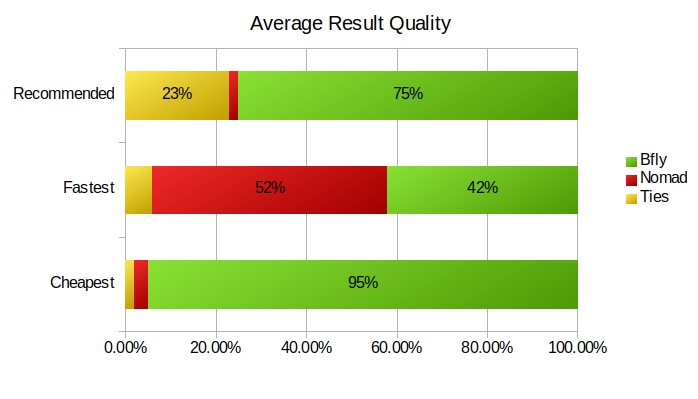
\includegraphics[width=8.5cm]{./imgs/average_result_quality.jpg}
    \caption{Comparison of the results provided by the proposed tool and by \textit{Kiwi}'s \textit{Nomad} application.}
    \label{fig:quality_apis}
\end{figure}

Fig.~\ref{fig:quality_apis} illustrates the obtained comparison, by presenting the total number of times that an application outperformed the other, for each of the three different optimization criteria. It also shows the number of cases in which the responses were very similar.

The analysis of this figure indicates that the developed application presents better solutions for a significant amount of queries. In fact, while the fastest set of flights is only achieved in 42\% of the queries, it presents the cheapest set of flights 95\% of the times and the best recommended result 75\% of the times. \todo{Nota: paragrafo abaixo}

Caso o professor considere apropriado, posso justificar a baixa taxa de sucesso do "fastest". Isto deve-se a uma ligeira falha na implementacao. Quando fazemos os pedidos dos dados dos voos, eu apenas guardo um subset da resposta, para poupar memoria. No entanto, eu escolho sempre o subset com o preco mais baixo. Logo, os voos mais rapidos perdem-se pelo caminho...


\subsection{Quantitative evaluation}
\label{sec:quantitative_eval}

To evaluate the difference of the responses provided by both applications, the total flight price and duration of the recommended set of flights was also quantitatively measured (see Fig.~\ref{fig:comparison}). The values presented in these graphs refer to the developed application response and were normalized using the \textit{Kiwi}'s \textit{Nomad} response as reference. 


\begin{figure}[h!]
\centering
    \begin{subfigure}[a]{0.5\textwidth}
      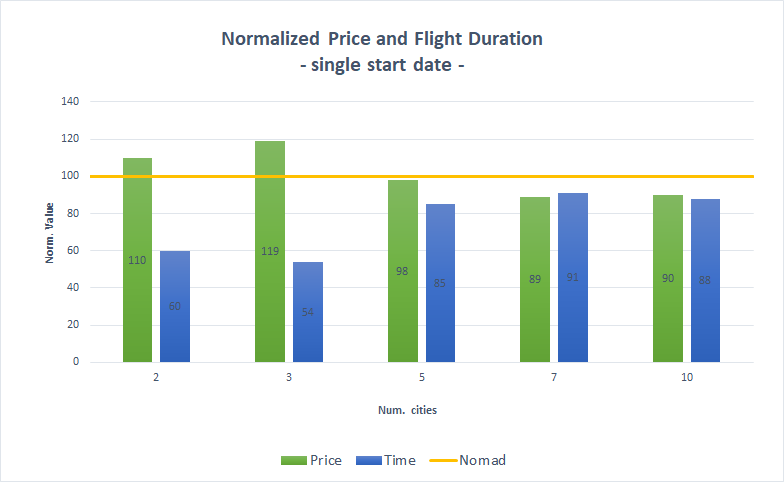
\includegraphics[width=1\linewidth]{./imgs/normalized_results_ss.png}
      \caption{Single start date.}
      \label{fig:comparison_a} 
    \end{subfigure}
    \begin{subfigure}[b]{0.5\textwidth}
      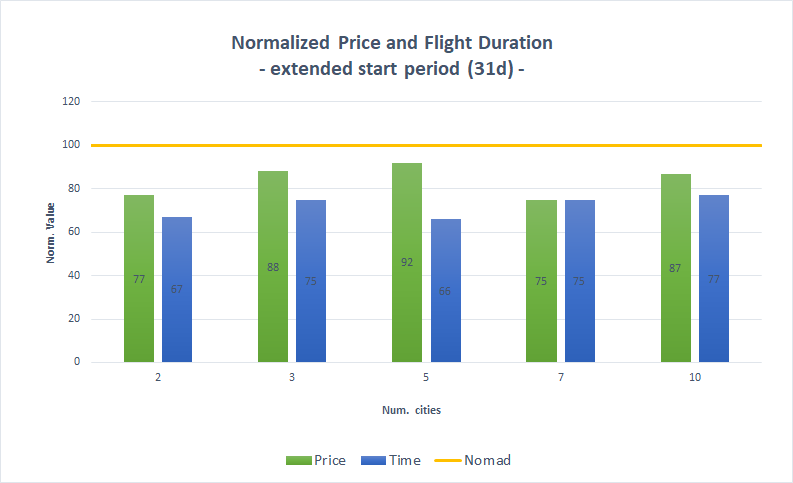
\includegraphics[width=1\linewidth]{./imgs/normalized_results_es.png}
      \caption{Extended start period (31 days).}
      \label{fig:comparison_b}
    \end{subfigure}
 \caption{Comparison of the recommended flights price and duration, as a function of the number of nodes and the length of start interval. The presented values refer to the proposed application response, and were normalized with respect to \textit{Kiwi}'s \textit{Nomad} response value.}
 \label{fig:comparison}
\end{figure}

Fig.~\ref{fig:comparison_a} presents the results of the queries performed for a single start date. Its analysis shows that, for a small number of nodes (2 and 3), the developed application recommends flights that are slightly more expensive ($\approx$ 10\% to 19\%) but have a much lower flight duration ($\approx$ 33\%-46\%). For requests with more nodes (5 to 10), the results presented by the developed application have both lower prices ($\approx$ 2\%-18\%) and flight duration ($\approx$ 9\%-24\%).

Figure ~\ref{fig:comparison_b} depicts the obtained results when the length of the start interval was extended to 31 days. With such an extended start period, every recommended set of flights provided by the proposed application has a lower price and duration. The price presents the most significant change: the minimum improvement is 8\%, while the maximum is 29\%.

Finally, it is worth noting that all the presented experiments only consider up to 10 different cities to be visited by the traveler. The reason why more nodes were not considered arises not from the developed application (which could easily accommodate more cities), but is motivated by a strict limit presented by \textit{Kiwi}'s \textit{Nomad} application, which does not support more than 10 nodes in the planned route.
  

% \subsubsection{Evaluating optimization performance}
% Given the more than 100 different queries considered, we compared the quality of the responses of both application for each optimization criteria. The results are presented in figure \ref{fig:quality_apis},
% and show that Bfly consistently present higher quality results, for both the cheapest, and the recommended set of flights. \textbf{Out of 100 different queries, Bfly presented the cheapest set of flights 95 times}, loosing three times to Kiwi, and tying two. As for the recommended set of flights, Bfly presents the better response 75 times, looses twice, and presents similar responses to Kiwi's 23 times. 

% \begin{figure}
%     \centering
%     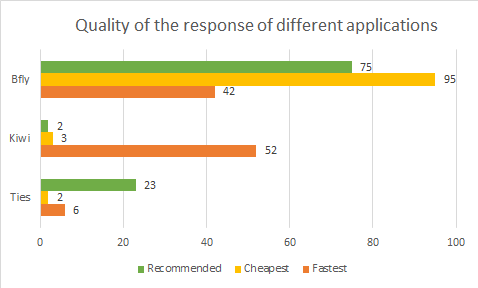
\includegraphics[width=8.5cm]{./imgs/quality_apis.png}
%     \caption{Comparison of the quality of the results of Bfly API, and Kiwi's \textit{Nomad} application.}
%     \label{fig:quality_apis}
% \end{figure}

% % We also analyzed the average quality improvement of Bfly compared to Kiwi's Nomad. These results are presented in table \ref{tab:kiwi_vs_bfly_1} and \ref{tab:kiwi_vs_bfly_15} for a single start date, and for a range of start dates (15 days), respectively. In both cases, Bfly consistently presents better results. For the extended start period, Kiwi wins only in 4 different occasions (2,5,8 and 9 nodes), and only for one optimization criteria (fastest trip). For the single start date, both applications present high quality responses for 2, 3 and 4 nodes. In these cases, one application presents better results for one criteria, but looses or ties in the other two criteria. As the number of nodes increases (5 to 10), Bfly reports better results for the cheapest and recommended set of flights.

% % \begin{figure}[h!]
% %     \centering
% %     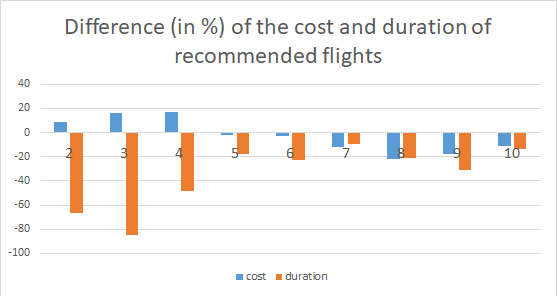
\includegraphics[width=8.5cm]{./imgs/recommended_1.png}
% %     \caption{Difference in flight cost and duration, for a single start date, as a function of the number of nodes.}
% %     \label{fig:quality_apis}
% % \end{figure}

% % \begin{figure}[h!]
% %     \centering
% %     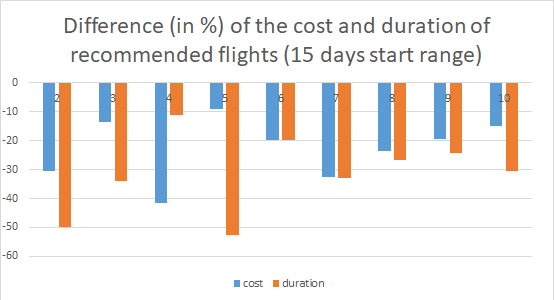
\includegraphics[width=8.5cm]{./imgs/recommended_15.png}
% %     \caption{Comparison of difference in flight cost and duration, for a range of start dates (15 days), as a function of the number of nodes.}
% %     \label{fig:quality_apis}
% % \end{figure}


% \begin{figure}
% \centering
% \begin{subfigure}[a]{0.5\textwidth}
%   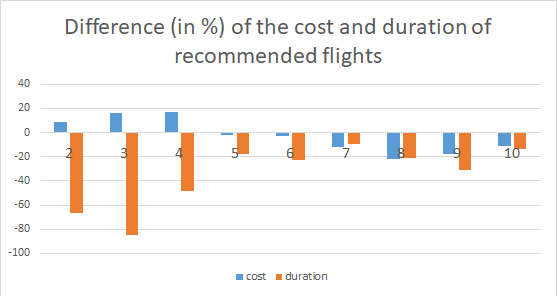
\includegraphics[width=1\linewidth]{./imgs/recommended_1.png}
%   \caption{}
%   \label{fig:Ng1} 
% \end{subfigure}

% \begin{subfigure}[b]{0.5\textwidth}
%   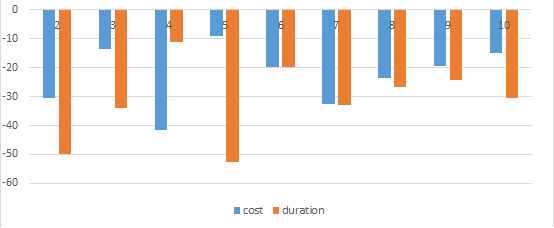
\includegraphics[width=1\linewidth]{./imgs/recommended_15_clean.png}
%   \caption{}
%   \label{fig:Ng2}
% \end{subfigure}

% \caption[asadadsa]{Difference, in \%, of the total cost and flight duration of the recommended set of flights, as a function of number of nodes. A negative value indicates that Bfly presents a lower value response, and thus, a positive result. (a) indicates queries with a single start date. (b) indicates queries with an extended start period (15 days).}
% \label{fig:recommended}
% \end{figure}

% Figure \ref{fig:recommended} enables the comparison of the total flight prices and duration between the responses of Kiwi and Bfly applications. The presented values are relative to that presented by Kiwi. Thus, a negative value in the price/duration indicates that Bfly presented a lower value response, and thus, a better result. This figure is also divided into two subplots, one for a single start date (a), and another for an extended start period (b). 

% From the analysis of figure \ref{fig:Ng1}, it can be seen that, for a low number of nodes (2, 3 and 4),
% Kiwi presents flights which are cheaper ($\approx$ 10-20\%), but slower ($\approx$ 40-80\%). However, for 5 to 10 nodes, Bfly presents results of higher quality. For 5 and 6 nodes, the cost improvement is not relevant ($\approx$ 2-3\%), but there is a considerable improvement in the flight duration ($\approx$ 20\%). As the number of nodes increases, so does the cost improvement ($\approx$ 10-20\%).

% In its turn, figure \ref{fig:Ng2} indicates that the overall quality of Bfly results improve for queries with an extended start period. First of all, Bfly always presents the better result, compared to Kiwi: for any number of nodes, the total flight duration and cost is lower. Furthermore, the cost improvement is considerably higher for extended start periods: the minimum improvement is $\approx$ 10\%, while the maximum is greater than 30\%. 


